\documentclass[a4paper 10pt]{article}
\usepackage[english,polish]{babel}
\usepackage[MeX]{polski}
\usepackage[utf8]{inputenc}
\usepackage[T1]{fontenc}
\usepackage[letterpaper, portrait, margin=1in]{geometry}
\usepackage{graphicx}
\usepackage{listings}
\usepackage{subfigure}
\usepackage{dashrule}
\usepackage{listings}
\usepackage{float}
\usepackage{amsmath}
\usepackage{listings}
\usepackage{multirow}
\usepackage{amsmath}
\usepackage{xcolor}
\usepackage{listings}
\usepackage{hyperref}
\hypersetup{ hidelinks = true, } 
\lstset{
    frame=single,
    breaklines=true,
    postbreak=\raisebox{0ex}[0ex][0ex]{\ensuremath{\color{red}\hookrightarrow\space}}
}


\renewcommand{\rmdefault}{ptm}
  
\frenchspacing

% Used to add additional dot in enumerations
\usepackage{titlesec}
\titlelabel{\thetitle.\quad}
\title{\textbf{Techniki Optymalizacji} \\
Laboratorium nr 3 \\
Sprawozdanie}
\author{Paulina Sadowska, Rafał Araszkiewicz}
\begin{document}
\maketitle

\section{Wprowadzenie}
Celem ćwiczenia było poprawienie wyników otrzymanych na ostatnich zajeciach  laboratoryjnych poprzez zastosowanie Multiple Start Local Search (Lokalne przeszukiwanie z różnych punktów startowych) oraz Iterated Local Search (Iteracyjne Przeszukiwanie Lokalne).
\section{Multiple Start Local search}
\label{Multiple Start Local search}
\subsection{Implementacja w pseudokodzie}
\begin{lstlisting}[frame=single]
powtorz 10 razy
	powtorz 1000 razy
		wygeneruj rozwiazania algorytmu NNG GCG lub Random dla losowego punktu startowego
		wykonaj Local Search
		jezeli wygenerowana trasa jest lepsza niz dotychczasowa najlepsza trasa
			bestPath = newPath;
	koniec
	dodaj bestPath do tabeli wynikow
koniec

\end{lstlisting}

\section{Iterated Local search}
\label{Iterated Local search}
Za preturbacje przyjęto złożenie dwóch zmian par wierzchołków, dwóch zmian par krawędzi, lub zmianę jednej pary wierzchołków i jednej pary krawędzi.
\subsection{Implementacja w pseudokodzie}
\begin{lstlisting}[frame=single]
wykonaj 10 razy
	wygeneruj rozwiazania algorytmu NNG GCG lub Random dla losowego punktu startowego
		dopoki nie uplynie zadany czas
			perturbancja = zlozenie dwoch zniam wierzcholkow lub krawedzi
			wykonaj perturbacje
			wykonaj Local Search
			
			jezeli koszt trasy po wykonaniu perturbacji i ruchu znalezionego przez LS jest wiekszy niz koszt sprzed ruchow
				przywroc poprzednia trase
		koniec
koniec
\end{lstlisting}

\section{Najlepsze ścieżki}
\subsection{Nearest Neighbour Grasp + Multiple Start Local Search}
Najlepsza trasa: 0, 62, 5, 48, 74, 96, 3, 64, 65, 69, 21, 15, 87, 78, 17, 23, 37, 35, 83, 9, 71, 20, 73, 58, 16, 14, 10, 31, 44, 90, 97, 22, 76, 59, 61, 34, 85, 26, 11, 19, 6, 8, 56, 86, 50, 24, 60, 57, 27, 92, 0 
\begin{figure} [H]
\centering
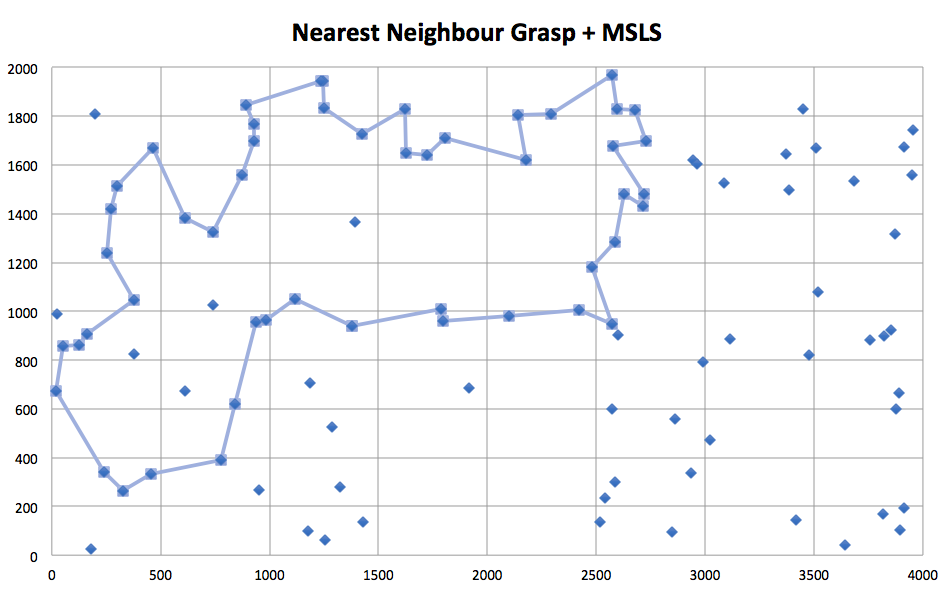
\includegraphics[angle=0,width = 1\textwidth, height=!]{images/NNG_MSLS.png}
\caption{Najlepsza trasa - Nearest Neighbour Grasp + Local Search}
\label{Rys. NN}
\end{figure}

\newpage
\subsection{Greedy Cycle Grasp + Multiple Start Local Search}
Najlepsza trasa: 59, 61, 34, 85, 26, 11, 19, 6, 8, 56, 86, 50, 24, 80, 60, 57, 66, 27, 92, 0, 91, 7, 55, 96, 18, 52, 87, 15, 69, 21, 93, 17, 23, 37, 83, 9, 89, 48, 5, 62, 46, 10, 16, 14, 31, 44, 90, 97, 22, 76, 59 
\begin{figure} [H]
\centering
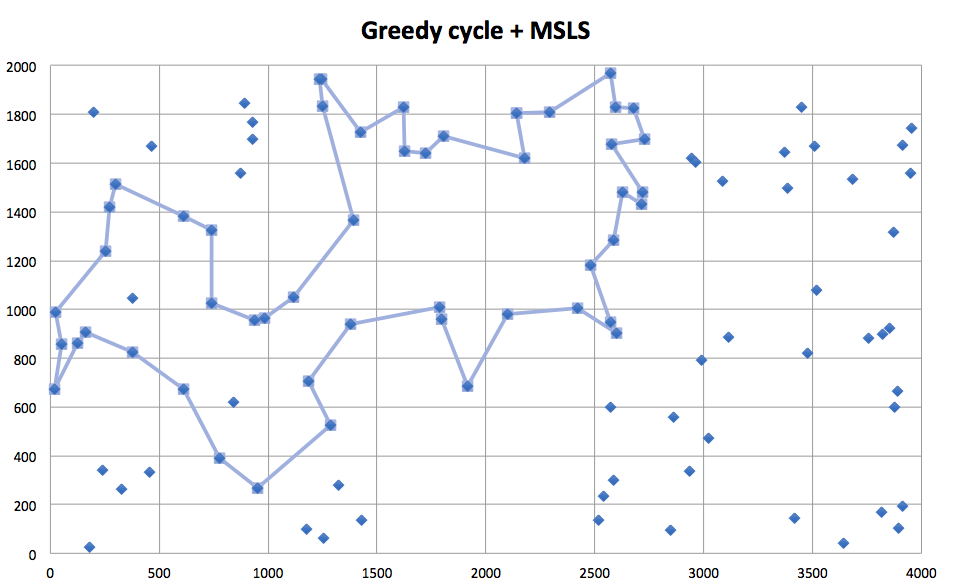
\includegraphics[angle=0,width = 1\textwidth, height=!]{images/GCG_MSLS.png}
\caption{Najlepsza trasa - Greedy Cycle Grasp + Local Search}
\label{Rys. NN}
\end{figure}
\newpage
\subsection{Random + Multiple Start Local Search}
Najlepsza trasa: 60, 57, 27, 92, 0, 62, 5, 48, 74, 18, 52, 87, 15, 21, 93, 78, 17, 23, 37, 35, 71, 20, 73, 16, 14, 10, 31, 44, 90, 97, 22, 59, 61, 85, 26, 11, 19, 56, 8, 6, 54, 82, 33, 45, 28, 29, 38, 84, 80, 24, 60 
\begin{figure} [H]
\centering
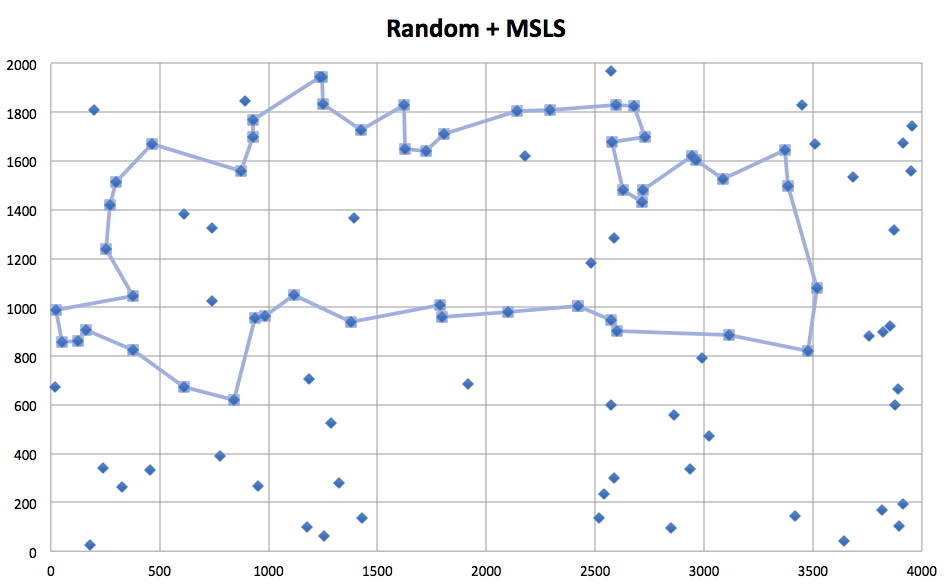
\includegraphics[angle=0,width = 1\textwidth, height=!]{images/Random_MSLS.png}
\caption{Najlepsza trasa - Random + Local Search}
\label{Rys. NN}
\end{figure}

\newpage
\section{Nearest Neighbour Grasp + Iterated Local Search}
Najlepsza trasa: 97, 90, 31, 10, 14, 16, 73, 20, 71, 83, 23, 17, 93, 21, 15, 87, 78, 52, 18, 65, 64, 3, 96, 55, 79, 30, 88, 41, 7, 91, 74, 48, 5, 62, 0, 92, 27, 66, 57, 60, 24, 50, 86, 56, 11, 26, 85, 34, 61, 59, 97 
\begin{figure} [H]
\centering
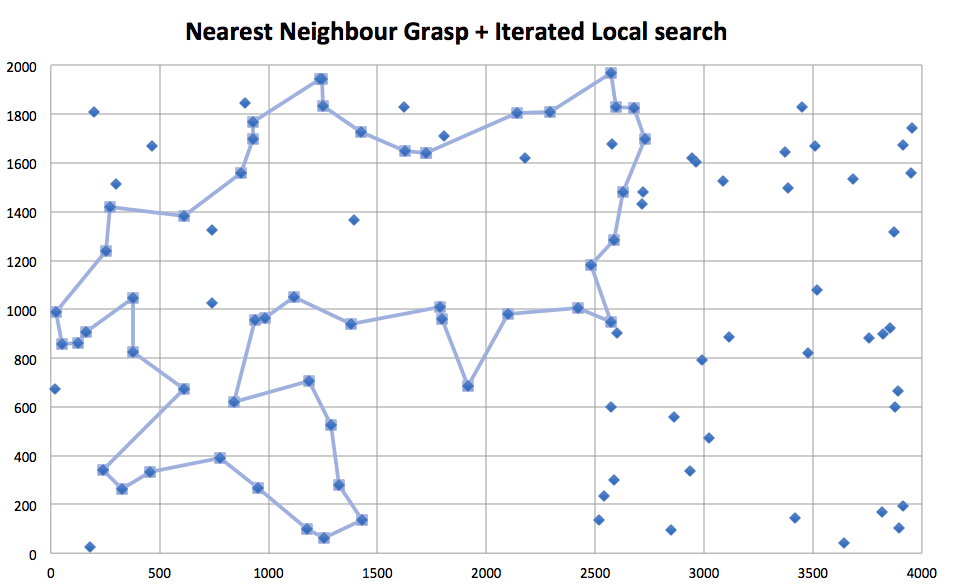
\includegraphics[angle=0,width = 1\textwidth, height=!]{images/NNG_ILS.png}
\caption{Najlepsza trasa - Nearest Neighbour Grasp + Iterated Local Search}
\label{Rys. NN}
\end{figure}

\newpage
\section{Greedy Cycle Grasp + Iterated Local Search}
Najlepsza trasa: 65, 69, 21, 15, 87, 93, 17, 23, 37, 98, 35, 83, 9, 71, 20, 73, 58, 16, 14, 10, 31, 44, 22, 97, 90, 46, 0, 92, 27, 57, 66, 88, 30, 79, 41, 7, 91, 62, 5, 48, 89, 78, 52, 18, 74, 55, 96, 3, 64, 25, 65 

\begin{figure} [H]
\centering
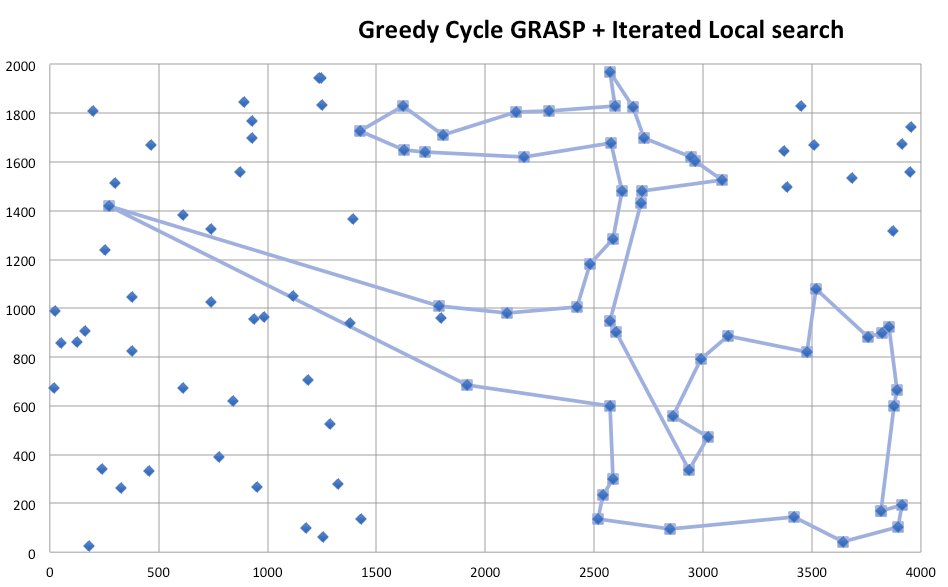
\includegraphics[angle=0,width = 1\textwidth, height=!]{images/GCG_ILS.png}
\caption{Najlepsza trasa - Greedy Cycle Grasp + Iterated Local Search}
\label{Rys. NN}
\end{figure}

\newpage
\section{Random + Iterated Local Search}
Najlepsza trasa: 91, 48, 5, 0, 66, 63, 39, 53, 1, 81, 12, 36, 4, 51, 77, 95, 38, 29, 28, 2, 45, 82, 54, 6, 8, 86, 50, 56, 19, 11, 26, 85, 61, 59, 76, 22, 97, 90, 44, 31, 20, 71, 9, 89, 74, 55, 79, 30, 41, 7, 91 

\begin{figure} [H]
\centering
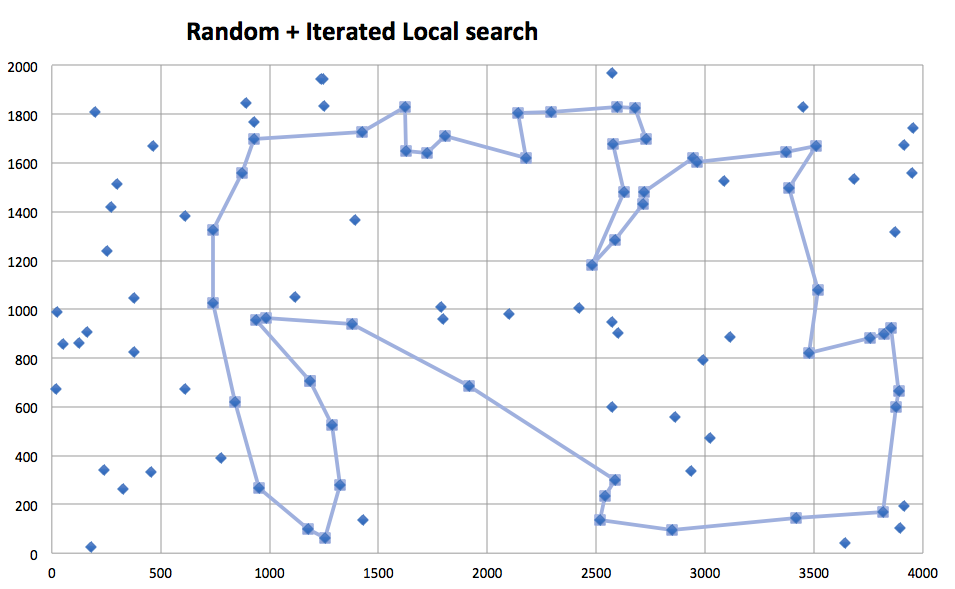
\includegraphics[angle=0,width = 1\textwidth, height=!]{images/Random_ILS.png}
\caption{Najlepsza trasa - Random + Iterated Local Search}
\label{Rys. NN}
\end{figure}

\newpage
\section{Otrzymane wyniki}
\begin{table}[H]
\centering
\caption{Otrzymane wyniki}
\label{my-label}
\begin{tabular}{|l|l|l|l|l|l|l|}
\hline
             & NNG + MSLS & GCG + MSLS & Random + MSLS & NNG + ILS & GCG + ILS & Random + ILS \\ \hline
min cost     & 9510 & 11548 & 10189 & 9483 & 9614 & 10553 \\ \hline
average cost & 9525 & 10549 & 10301 & 9522 & 9806 & 11400 \\ \hline
max cost     & 9664 & 10551 & 10375 & 9698 & 10034 & 11694 \\ \hline
best time    & 36.4s & 10.1s & 52.6s & 41.1s & 11.1s & 61.1s \\ \hline
average time & 41.1s & 11.1s & 61.1s & 41.1s & 11.1s & 61.1s \\ \hline
worst time   & 46.2s & 11.9s & 69.8s & 41.2s & 11.1s & 61.1s \\ \hline 
\end{tabular}
\end{table}
\end{document}
\\